\mychapter{Equacions i sistemes d'equacions}{Equacions i sistemes}{}{chap:equacions}
  \vso
  
\begin{iniaval}
	\textbf{Resol les següents equacions}
	
	\begin{tasks}(2)
		\task  $\boldsymbol{2}\boldsymbol{x}\boldsymbol{+}\boldsymbol{5}\boldsymbol{=}\boldsymbol{2}\boldsymbol{-}\boldsymbol{x}$
		
		
		\task
		$ \boldsymbol{2}\left(\boldsymbol{x}\boldsymbol{-}\boldsymbol{1}\right)\boldsymbol{=}\boldsymbol{3}\boldsymbol{-}\boldsymbol{(}\boldsymbol{1}\boldsymbol{-}\boldsymbol{x}\boldsymbol{)}$ 
		
		\vso
		\vso
	 	
		
		\task
		${\boldsymbol{x}}^{\boldsymbol{2}}\boldsymbol{+}\boldsymbol{5}\boldsymbol{x}\boldsymbol{+}\boldsymbol{4}\boldsymbol{=}\boldsymbol{0}$
		
		
		\task \textbf{Què val cada fruita?}
		
		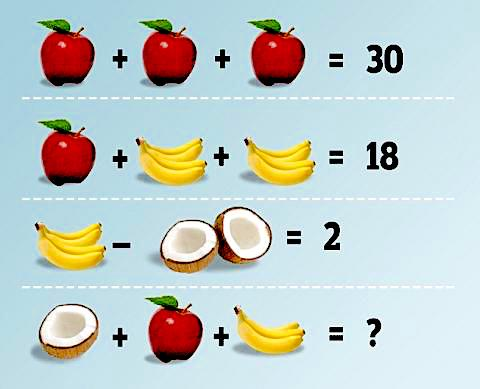
\includegraphics[width=0.43\textwidth]{img-06/tutifruti}
		
		
	\end{tasks}
	\vso
	
	
	\addanswersline[cols=1]{Avaluació inicial}{0}{[$x=-1$, $x=4$, $x=-4$, cirera=9 punts i síndria=11 punts]}
\end{iniaval}



\pagebreak

\section{ Concepte d'equació }

\begin{mylist}




\exer  La balança de la figura està equilibrada. Què pesa un quadrat si sabem que les boles grosses fan 2 kg i les petites 1 kg?

\begin{center}
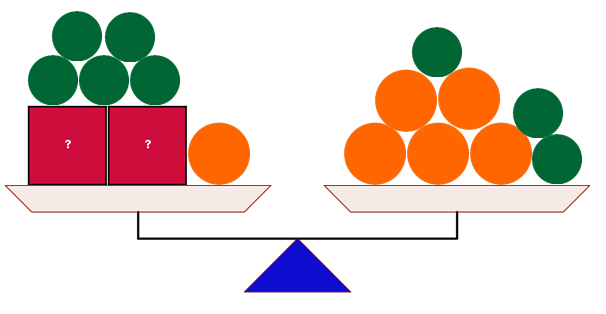
\includegraphics[width=6cm]{img-06/balanza02}
\end{center}

Si anomenam $x$ al pes d'un quadrat, podries plantejar una equació per resoldre el problema?

\answers{$2x+5+2=3+10$, aïllam $x$,\par $2x=13-7$\par $x=\frac{6}{2}=3$ kg cada quadrat}

\begin{comment}
\exer  Copia en el teu quadern la següent taula i completa-la:

\begin{center}
	\renewcommand*{\arraystretch}{1.2}
\begin{longtable}{|p{1.2in}|p{1.2in}|p{1.2in}|p{1.2in}|} \hline 
\textbf{Equació} & \textbf{Primer membre} & \textbf{Segon membre} & \textbf{Incògnites} \hline 
8\textit{x} -- 1 = 4\textit{x} -- 7 &  &  &  \hline 
 & 5\textit{x} + 9 & 3\textit{x} -- 1 &  \hline 
2\textit{a +} 3 = 32 &  &  &  \hline 
 & 2\textit{x} -- 5\textit{y} & 5 + 4\textit{y} &  \hline 
\end{longtable}
\end{center}
\end{comment}

\exer \mental Indica el nombre d'incògnites de les següents equacions:
\begin{tasks}(2) 
	\task  4 \textit{x} -- 5\textit{y =} 7\textit{x} + 6  
	\task  2\textit{x }+ 8\textit{y${}^{2}$ }= 5  
	\task  3\textit{a + }6\textit{a${}^{ }$}${}^{2}$ = 3  
	\task  4\textit{x }+ 8\textit{x${}^{2}$ }= 12
\end{tasks}

\answers{[Una incògnita, Dues incògnita, Una incògnita, Una incògnita]}

\exer \mental  Indica el grau de les següents equacions:

\begin{tasks}(2)
	\task  2\textit{x} -- 4 = 6\textit{x} + 8   
	\task  3\textit{x} + 9\textit{y${}^{2}$ }= 12  
	\task  5\textit{x} + 10\textit{x${}^{2}$ }= 30  
	\task  2\textit{x} + 2\textit{xy${}^{2}$ }= 3
\end{tasks}

 \answers{[Primer grau, Segon grau, Segon grau, Tercer grau]}

\end{mylist}



\section{Equacions de primer grau}

\begin{theorybox}[Transposar termes]
	\begin{tabular}{llcl}
{\normalfont\it Si és positiu passa negatiu} & $x \, \boxed{+3}=5$ & $\rightarrow$ & $x=5-3$ \\  
{\normalfont\it Si negatiu passa positiu} & $x \, \boxed{-3}=5$ & $\rightarrow$ & $x=5+3$ \\  
{\normalfont\it Si multiplica la $x$ passa dividint} & $\boxed{3} \, x=15$ & $\rightarrow$ & $x=\frac{15}{3}$ \\  
{\normalfont\it Si divideix la $x$ passa multiplicant} & $\frac{x}{\boxed{2}}=8$ & $\rightarrow$ & $x=2\cdot 8$ \\  
\end{tabular}
\end{theorybox}

\begin{mylist}
\exer  \spen Resol aquestes equacions aquí.

\begin{tasks}(2) 
	\task  ${ 4x}={ 20}$      
	\task  $x+{ 3}={ 5}$    
	\task  $x-{ 1}=-{ 8}$    
	\task  $3x=12$     
	\task  $\frac{x}{{ 3}} ={ 2}$     
	\task  $x+{ 4}={ 8}$     
\end{tasks}

\answers{[$x=5$, $x=2$, $x=-7$, $x=4$, $x=6$, $x=4$]}

\pagebreak

\exer[1]  Resol:
\begin{tasks}(2)
	\task ${ 2x}-{ 1}=x+{ 2}$                  
	\task ${ 3x}+{ 2}=x+{ 6}$                     
	\task ${ 2x}+{ 1}={ 5x}-{ 5}$                   
	\task ${ 1}-x={ 4}-{ 2x}$                  
	\task $x-{ 6}={ 5x}-{ 2}$                      
	\task ${ 3}+{ 7x}={ 2x}+{ 5}$ 
	\task ${ 6x}-{ 2}+x={ 2x}+{ 3}$        
	\task ${ 8x}+{ 3}-{ 5x}={ 7}-{ 2x}-{ 1}$      
	\task ${ 4x}+{ 5}+x={ 7}+{ 3x}-{ 3}$ 
	\task ${ 8}-x+{ 1}={ 4x}-{ 1}-{ 7x}$     
	\task ${ 7x}-{ 4}-{ 3x}={ 2}+{ 4x}-{ 6}$     
	\task ${ 2}+{ 3x}-{ 5}={ 4x}-{ 2}-x$
\end{tasks}

\answers[cols=4]{[3, 2, 2, 3, --1, 2/5, 1, 3/5, -1/2, -5, I.S., S.S.]} 


\end{mylist}

\begin{minipage}{0.4\textwidth}
	\begin{example}
		\begin{tabular}{rcl}
			a) \quad\quad\quad  ${ 2x}-{ 1}$ &=& $x+{ 2}$ \\
			$ 2x-x$ &=& $2+1$ \\
			$ x$ &=& $\boxed{3}$ \\
			
		\end{tabular}
	\end{example}
\end{minipage}
\hspace{0.5cm}
\begin{minipage}{0.5\textwidth}
	\vspace{0.3cm}
	\begin{warningbox}
		Si trobes $0\cdot x = 0$ \, $\rightarrow$ \, Té $\infty$ solucions.
		\vspace{0.4cm}
		
		Si trobes $0\cdot x = 1$ \, $\rightarrow$ \, No té cap solució.
		
	\end{warningbox}
\end{minipage}

\begin{mylist}

\exer[1] Resol en cada cas:

\begin{tasks}(2)
	\task  ${ 1}-{ 2}({ 2x}-{ 1})={ 5x}-({ 5}-{ 3x})$                        
	\task $x-\left({ 1}-{ 3x}\right)={ 8x}-{ 1}$                      
	\task  ${ 1}-({ 3x}-{ 9})={ 5x}-{ 4x}+{ 2}$          
	\task ${ 13}x-{ 15}-{ 6x}={ 1}-({ 7x}+{ 9})$      
	\task ${ 7x}-({ 4}+{ 2x})={ 1}+(x-{ 2})$           
	\task ${ 2}({ 3x}-{ 1})-{ 5x}={ 5}-({ 3x}+{ 11})$   
	\task  $x-{ 7}={ 6}-(x-{ 3})$      
	\task ${ 7}-({ 2x}+{ 9})={ 11}x-{ 5}({ 1}-x)$         
	\task ${ 4}({ 5x}-{ 3})-{ 7x}={ 3}({ 6x}-{ 4})+{ 10}$        
	\task ${ 4}-{ 7}({ 2x}-{ 3})={ 3x}-{ 4}({ 3x}-{ 5})$   
	\task ${ 16}x-{ 7}(x+{ 1})={ 2}-{ 9}({ 1}-x)$            
	\task ${ 6}-({ 8x}+{ 1})={ 4x}-{ 3}({ 2}+{ 4x})$
\end{tasks}
\answers[cols=4]{[2/3, 0, 2, 1/2, 3/4, --1, 8, 1/6, --2, 1, I.S., S.S.]}

\end{mylist}

\begin{example}
	\begin{tabular}{lrcl}
		a) \quad\quad\quad\quad\quad\quad\quad\quad\quad\quad\quad & $1-2(2x-1)$ &=& $5x-(5-3x)$ \\
		Eliminam parèntesis & $ 1-4x+2$ &=& $5x-5+3x$ \\
		Transposam termes& $ -4x-5x-3x$ &=& $-5-1-2$ \\
		Simplificam & $-12x$ &=& $-8$ \\
		Canviam signes& $12x$ &=& $8$ \\
		Solució & $x$ &=& $\frac{8}{12}=\boxed{\frac{2}{3}}$ \\
	\end{tabular}
\end{example}


\begin{mylist}
	

\exer[1]  Resol al teu quadern les següents equacions amb denominadors:
\begin{tasks}(2)
	\task ${ 1}+\frac{{ 2x}}{{ 5}} =\frac{{ 1}}{{ 5}} -{ 2x}$                                         
	\task  $\frac{{ 2x}}{{ 3}} +\frac{{ 5}}{{ 3}} =\frac{{ 1}}{{ 3}} $                    
	\task  ${ 4}-\frac{{ 2x}}{{ 3}} =x+\frac{{ 2}}{{ 3}} $              
	\task   $\frac{x}{{ 5}} +\frac{{ 1}}{{ 5}} =\frac{{ 4}}{{ 5}} $ 
	\task  $\frac{{ 1}}{{ 4}} -x=\frac{{ 3x}}{{ 4}} -{ 1}$           
	\task  $\frac{{ 3x}}{{ 2}} +{ 5}={ 2x}-\frac{{ 1}}{{ 2}} $           
\end{tasks}
\answers[cols=4]{[--1/3, --2, 2, 3, 5/7, 11]} 

\end{mylist}

\begin{example}
	\begin{tabular}{lrcl}
		a) \quad\quad\quad\quad\quad\quad\quad\quad\quad\quad\quad & ${ 1}+\frac{{ 2x}}{{ 5}}$ &=& $\frac{{ 1}}{{ 5}} -{ 2x}$  \\[0.25cm]
		Multiplicam tot pel mcm=5 & $5\cdot{ 1}+5\cdot\frac{{ 2x}}{{ 5}}$ &=& $5\cdot\frac{{ 1}}{{ 5}} -5\cdot{ 2x}$ \\[0.25cm]
		Eliminam denominadors & $5 +2x$ &=& $1 -10x$ \\ [0.25cm]
		Transposam termes& $ 2x+10x$ &=& $1-5$ \\[0.15cm]
		Simplificam & $12x$ &=& $-4$ \\[0.15cm]
		Solució & $x$ &=& $\frac{-4}{12}=\boxed{\frac{-1}{3}}$ \\
	\end{tabular}
\end{example}


\begin{mylist}

\exer[1]  Resol en cada cas:

\begin{tasks}(2)
	\task  $\frac{{ 3x}}{{ 4}} +\frac{{ 2x}}{{ 5}} +\frac{x}{{ 10}} ={ 1}$            
	\task  $\frac{{ 3x}}{{ 2}} -\frac{{ 1}}{{ 5}} =\frac{{ 3x}}{{ 5}} -\frac{{ 1}}{{ 2}} $           
	\task  $\frac{x}{{ 2}} +\frac{{ 1}}{{ 3}} =\frac{x}{{ 3}} +\frac{{ 1}}{{ 4}} $         
	\task  $\frac{x}{{ 2}} -\frac{{ 5}}{{ 6}} =\frac{x}{{ 3}} -\frac{x}{{ 5}} +{ 1}$  
	\task $x-\frac{{ 3x}}{{ 4}} +\frac{{ 1}}{{ 10}} =\frac{{ 4x}}{{ 5}} -\frac{x}{{ 2}} $           
	\task   $\frac{x}{{ 2}} +\frac{{ 1}}{{ 6}} -\frac{x}{{ 3}} =\frac{x}{{ 6}} -\frac{{ 2}}{{ 3}} +\frac{{ 5}}{{ 6}} $      
\end{tasks}
\answers[cols=4]{[4/5, --1/3, --1/2, 5, 2, I.S., S.S.]} 




\exer  Resol les següents equacions de primer grau amb denominadors:

\begin{tasks}(2)
	\task  $\frac{x-1}{2} -\frac{x+1}{3} =10$   
	\task   $\frac{x-3}{3} +\frac{-x+1}{7} =3$  
	\task  $\frac{x+1}{5} +\frac{2x+6}{10} =2$
	\task  $\frac{1-x}{2} +\frac{3x-1}{3} =\frac{1}{3} $   
	\task  $\frac{2x-8}{5} -\frac{3x-9}{10} =x-1$  
	\task  $\frac{2x+3x}{5} -\frac{3x-6}{10} =1$
\end{tasks}

\answers{[$x=65$, $x=\frac{81}{4}$, $x=3$, $x=\frac{1}{3}$, $x=\frac{1}{3}$, $x=\frac{4}{7}$]}

\end{mylist}

\begin{example}
	\begin{tabular}{lrcl}
		a) \quad\quad\quad\quad\quad\quad\quad\quad\quad\quad\quad & $\frac{x-1}{2} -\frac{x+1}{3}$ &=& $10$  \\[0.25cm]
		Multiplicam tot pel mcm=6 & $6\cdot\frac{(x-1)}{2} -6\cdot\frac{(x+1)}{3}$ &=& $6\cdot 10$ \\[0.25cm]
		Eliminam denominadors & $3\cdot(x-1) -2\cdot(x+1)$ &=& $60$ \\ [0.25cm]
		Eliminam parèntesis & $3x-3 -2x-2$ &=& $60$ \\ [0.25cm]
		Transposam termes& $ 3x-2x$ &=& $60+2+3$ \\[0.15cm]
		Reduïm & $x$ &=& $\boxed{65}$ \\[0.15cm] 
	\end{tabular}
\end{example}


\pagebreak
\subsection{Problemes d'equacions de primer grau}

\begin{mylist}
\exer  La tercera part de la meva edat sumada a la seva meitat són 15 anys. Quina edat tinc?  

\answers{Anomenam $x$: La meva edat. Plateig: $\frac{x}{3}+\frac{x}{5}=15$. Solució $x=18$ anys}

\exer  Un empleat d'un concessionari de cotxes guanya 850 euros cada mes, més un plus de 53 euros per cada cotxe que ven. Quants cotxes ha venut si en total aquest mes ha guanyat 1.221 euros? 

\answers{Anomenam $x$: num. de cotxes. Plateig: $850+53x=1221$. Solució $x=7$ cotxes} 

\exer  A una caminada popular hi participen 16 dones més que homes. Si en total hi han participat 204 persones, quants homes i quantes dones hi han participat? 

\answers{Anomenam $x$: homes i $x+16$ dones. Plateig: $x+x+16=204$. Solució $x=94$ homes i $110$ dones}

\exer  El meu germà té 10 euros menys que jo, i la meva germana, el doble que el meu germà. Entre tots tenim 470 euros. Quants euros té cadascun? 

\answers{Anomenam $x$: \euro{} jo; $x-10$ germà; $2(x-10)$ germana. Plateig: $x+x-10+2(x-10)=470$. Solució $x=125$ \euro{} jo; 115 \euro{} germà; 230 \euro{} germana }

\exer  El triple de l'edat que tenia en Jordi fa 4 anys és el doble de la que tindrà d'aquí a 8 anys. Quina és l'edat actual d'en Jordi? 

\answers{Anomenam $x$: edat actual Jordi; $x-4$: edat fa 4 anys; $x+8$: edat d'aquí 8 anys. Plateig: $3(x-4)=2(x+8)$. Solució $x=28$ anys}
 
\exer[1]  En la primera prova d'una oposició queda eliminat el 53\% dels participants. En la segona prova, s'elimina al 25\% dels restants. Si el nombre total de persones suspeses és de 518, quantes persones es van presentar a l'oposició?
 \answers{En total 800 persones. Suspenen 424 en la primera prova i 94 en la segona.}
 
\exer  En un rectangle, un costat és quatre vegades més gran que l'altre, i el perímetre és 100 cm. Calcula les longituds de cada costat.

\answers{Anomenam $x$: un costat; $4x$ l'altre costat. Plateig: $x+x+4x+4x=100$. Solució $x=10$ cm i $40$ cm.}
 
\exer  El perímetre d'un rectangle és 26 cm. Si la base mesura 3 cm més que l'altura, quines són les dimensions del rectangle? 

\answers{Anomenam $x$: altura; $x+3$ base. Plateig: $x+x+x+3+x+3=26$. Solució $x=5$ cm altura i base 8 cm.}

\exer  Hem de repartir 152 cromos entre tres nens, de manera que el segon en tingui 8 més que el primer i que el tercer en tingui 16 més que el segon. Com ho farem? 

\answers{Anomenam $x$: cromos 1r nen; $x+8$ el segon; $x+8+16$ el tercer. Plateig: $x+x+8+x+8+16=152$. Solució $x=40$ cromos al primer; 48 al segon; 64 al tercer.}

\exer[1] Per comprar 7 discos compactes em falten 12 €, però si només compro 5, em sobren 18 €. Si tots els compactes valen igual, quant en val un? 
\answers{cada disc 15 \euro{}; total 93 \euro{}}

\exer  En una competició d'atletisme hi ha el doble d'atletes dels EUA que d'Alemanya. Si en total hi ha 213 atletes, quants participants hi ha de cada un d'aquests dos països? 
\answers{Anomenam $x$: Atletes Alemanya i $2x$ atletes EUA. Plateig: $x+2x=213$. Solució $x=71$ atletes d'Alemanya i 142 d'EUA.}

\exer[1]  Una prova consta de 20 qüestions. Per cada qüestió contestada correctament, un alumne guanya 3 punts; però per cada qüestió contestada malament o no contestada, en perd 2. Si al final de la prova un alumne va aconseguir 30 punts, quantes qüestions va contestar correctament?
\answers{14 bé i 6 malament} 

\exer[1]  Tinc 20 monedes, unes de 0,50 euros i altres de 2 euros. Quantes monedes tinc de cada si sumen un total de 22 euros?
\answers{12 monedes de 0.50 \euro{} i 8 monedes de 2 \euro{}} 

\exer[1] Un dromedari té un gep, i un camell en té dos. En un ramat de camells i dromedaris hem comptat 86 caps i 148 geps. Quants camells i dromedaris hi ha? 
\answers{24 dromedaris i 62 camells}

\exer[1]  En arribar 32 persones a una reunió s'observa que ara el nombre d'assistents és igual al triple dels que hi havia menys 14. Quantes persones hi havia inicialment a la reunió? 
\answers{23 persones}

\end{mylist}


\section{Equacions de segon grau}

\begin{theorybox}
	\begin{multicols}{2}
		\centering
 \videonw[ytid=o1OZj3A8qb4]{26}{Equacions de 2n grau completes}
 \videonw[ytid=HA9ZB75NPJw]{23}{Equacions de 2n grau incompletes}
 \end{multicols}
 
 \textbf{ Equació de 2n grau completa: } $ax^2+bx+c\ =\ 0$.  
 \begin{center}
 Fórmula: $\boxed{ x=\frac{-b\pm \sqrt{b^2-4\cdot  a\cdot  c}}{2a} }$
 \end{center}
  \textbf{Discriminant} $\Delta =b^2-4\cdot a \cdot c$. 
 
 Si $\Delta >0$ té dues solucions diferents. Si $\Delta =0$ té una solució doble. Si $\Delta <0$ no té solució.
 
 \textbf{Exemples:}
 
 L'equació $x^2-x+3=0$ té discriminant $\Delta ={(-1)}^2-4\cdot1\cdot3=-11$ és negatiu, aleshores no té cap solució.
 
 L'equació${\ x}^2+2x+1=0$ té discriminant $\Delta =2^2-4\cdot1\cdot1=0$  és zero, aleshores té una solució repetida.
 
 L'equació${\ x}^2-5x+6=0$ té discriminant $\Delta ={(-5)}^2-4\cdot1\cdot6=1$  és positiu, aleshores té dues solucions diferents.
 

\end{theorybox}


\begin{mylist}
\exer  \mental Indica si són de segon grau les següents equacions:
\begin{tasks}(2)
 \task $5x^{2} -\sqrt{2} x+8=0$  \task  8\textit{x}${}^{2}$ $-$ 9 = 0   \task  $2x^{2} -\frac{3}{x} =0$ 
\task  3\textit{xy}${}^{2}$ $-$ 5 = 0    \task  8 $-$ 7,3\textit{x} = 0   \task  $2x^{2} -3\sqrt{x} +4=0$
 \end{tasks}

\answers{[Si, Sí, No. 3r grau, No. 3r grau, No. 1r grau, No]}

\exer  En les següents equacions de segon grau, indica què valen $a$, $b$ i $c$. 
	Calcula el discriminant i digues quantes solucions tenen.

\begin{tasks}(2) 
	\task  3 + 4\textit{x}${}^{2}$ + 5\textit{x} = 0   
	\task  $-$3\textit{x}${}^{2}$ + 5\textit{x} = 0   
	\task  2\textit{x}${}^{2}$ $-$ 3 = 0   
	\task  4\textit{x}${}^{2}$ $-$ 4\textit{x} + 1= 0
\end{tasks}

\answers[cols=1]{[ $a=4$,\;$b=5$ i $c=3$; $\Delta=-23<0$; Cap solució,
			$a=-3$,\;$b=5$ i $c=0$; $\Delta=5>0$; Dues solucions,
		$a=2$,\;$b=0$ i $c=-3$; $\Delta=24$; Dues solucions,
		$a=4$,\;$b=-4$ i $c=1$; $\Delta=0$; Una solució doble]}

\end{mylist}

\begin{example}
	a)	$3 + 4\textit{x}^{2} + 5\textit{x} = 0$ primer convé ordenar l'equació de major a menor grau:
		
		$4x^2+5x+3=0$  \quad  \quad $\rightarrow$  \quad \quad $a=4$, $b=5$ i $c=3$.
		
			
		El discriminant és $\Delta = 5^2 - 4 \cdot 4 \cdot 3 = -23$, negatiu llavors no té solució.	
\end{example}



\pagebreak


\begin{mylist}
	
\exer  Esbrina quantes solucions tenen les següents equacions de 2n grau:
\begin{tasks}(2)
	\task  \textit{x}${}^{2}$ + \textit{x} + 4 = 0    
	\task  \textit{x}${}^{2}$ $-$ 6\textit{x} + 9 = 0   
	\task  \textit{x}${}^{2}$ $-$ 6\textit{x} $-$ 7 = 0  
	\task \textit{ x}${}^{2}$ $-$ 3\textit{x} + 5 = 0
\end{tasks}

\answers{[Cap, $x=3$, $x=-1$ i $x=-7$, Cap]}

\exer  Resol les següents equacions de 2n grau completes:

\begin{tasks}(2)
	\task  \textit{x}${}^{2}$ $-$ 7\textit{x} + 10 = 0   
	\task  2\textit{x}${}^{2}$ + 2\textit{x} $-$ 24 = 0   
	\task  3\textit{x}${}^{2}$ $-$ 9\textit{x} + 6 = 0  
	\task \textit{ x}${}^{2}$ $-$ 4\textit{x} $-$ 12 = 0
\end{tasks}

\answers{[$x=2$ i $x=5$, $x=-4$ i $x=-3$, $x=1$ i $x=2$, $x=-2$ i $x=6$]}

\end{mylist}

\begin{example}
	a) \textit{x}${}^{2}$ $-$ 7\textit{x} + 10 = 0   
	
	Sabem que $a=1$, $b=-7$ i $c=10$
	
	$x=\frac{-(-7)\pm \sqrt{(-7)^2-4\cdot  1\cdot  10}}{2\cdot 1}=\frac{7\pm \sqrt{9}}{2}=\frac{7\pm 3}{2}=\left\{ \begin{array}{l} \frac{7 + 3}{2}=\boxed{5} \\ [0.25cm] \frac{7- 3}{2}=\boxed{2} \end{array} \right.$
	
\end{example}


\begin{theorybox}[ Equacions de segon grau incompletes]

 \textbf{Falta la \textit{b}},  $ax^2+c=0$:  Aïllar la $x$ i fer l'arrel quadrada $x=\pm \sqrt{-\frac{c}{a}}$.
 
 
  \textbf{Falta la \textit{c}},  $ax^2+bx=0$:  Treure $x$ factor comú. Les solucions són $x=0$ i $x=-\frac{b}{a}$  .
\end{theorybox}
 

 
\begin{mylist}

\exer[1]  Resol les següents equacions de 2n grau incompletes:

\begin{tasks}(2)
	\task  3\textit{x}${}^{2}$ + 6\textit{x} = 0    
	\task  3\textit{x}${}^{2}$ $-$ 27 = 0   
	\task  \textit{x}${}^{2}$ $-$ 25 = 0   
	\task  2\textit{x}${}^{2}$ + \textit{x} = 0    
	\task  4\textit{x}${}^{2}$ $-$ 9 = 0    
	\task  5\textit{x}${}^{2}$ $-$ 10\textit{x} = 0
\end{tasks}
\answers[cols=2]{[$x=0$ i $x=-2$, $x=\pm 3$, $x=\pm 5$, $x=0$ i $x=-1/2$, $x=-3/2$, $x=0$ i $x=2$]}

\end{mylist}

\begin{example}
	
	a) 3\textit{x}${}^{2}$ + 6\textit{x} = 0 \quad\quad   $\rightarrow$ \quad\quad $3x \cdot ( x+2)=0$ $\rightarrow$ \quad\quad $x=0$ i $x=-2$
	
	b) 3\textit{x}${}^{2}$ $-$ 27 = 0   \quad\quad   $\rightarrow$ \quad\quad $x^2 = 27/3 = 9$ $\rightarrow$ \quad\quad $x=-3$ i $x=3$
	
\end{example}


\begin{mylist}
	

\exer \mental  Resol mentalment les següents equacions de 2n grau:

\begin{tasks}(2)
	\task  \textit{x}${}^{2}$ + 6\textit{x} = 0    
	\task  \textit{x}${}^{2}$ + 2\textit{x} $-$ 8 = 0   
	\task  \textit{x}${}^{2}$ $-$ 25 = 0 
	\task  \textit{x}${}^{2}$ $-$ 9\textit{x} + 20 = 0   
	\task  \textit{x}${}^{2}$ $-$ 3\textit{x} $-$ 4 = 0   
	\task  \textit{x}${}^{2}$ $-$ 4\textit{x} $-$ 21= 0
\end{tasks}

\answers{[$x=0$ i $x=-6$, $x=-4$ i $x=2$, $x=-5$ i $x=5$, $x=4$ i $x=5$, $x=-1$ i $x=4$, $x=-3$ i $x=7$]}

\exer  El perímetre d'un rectangle mesura 16 cm i la seva àrea 15 cm${}^{2}$. Calcula les seves dimensions.

\answers{$x+y=16/2=8$ i $x\cdot y =15$. Els costats han d'ésser 5 i 3 cm}

\exer  Si 3 és una solució de ${x}^{2}- 5x + a= 0$, quant val \textit{a}?

\answers{${3}^{2}- 5\cdot 3 + a= 0$ aleshores $a=6$}

\end{mylist}

\subsection{Problemes d'equacions de segon grau}

\begin{mylist}
	
	
	\exer  Quin nombre multiplicat per 3 és 40 unitats menor que el seu quadrat?
	
	\answers{$3x+40=x^2$, poden ésser $x=-5$ o $x=8$}
	
	\exer  Calcula tres nombres consecutius tals que la suma dels seus quadrats sigui 365.
	
	\answers{$x^2+(x+1)^2+(x+2)^2=365$, queda l'equació de segon grau $3x^2+6x-360=0$ que té dues solucions $x=10$i $x=-12$. Els nombres poden ésser:
	\{10, 11, 12\} o bé \{-12, -11, -10\} }
	
	\exer  El triple del quadrat d'un nombre més el seu doble és 85. Quin és el nombre?
	
	\answers{$3x^2+2x=85$, el nombre és $x=5$ o $x=-\frac{17}{3}$}
	
	\exer  Un triangle isòsceles té un perímetre de 20 cm i la base mesura 4 cm, calcula els costats del triangle i la seva àrea.
	
	\answers{És un problema de 1r grau. Anomenam $x$ al costat igual del triangle. $2x+4=20$, que dóna $x=8$ cm. L'altura del triangle per Pitàgores 
		$h=\sqrt{8^2-2^2}=7.746$ cm l'àrea és $A=15.492$ cm$^2$}
\end{mylist}	


\section{ Equacions biquadrades i factoritzades}


\begin{theorybox}

 Una equació factoritzada és el producte de diferents termes igualat a zero.
 
 \begin{center}
 \textbf{                                     
	(Una cosa) · (Altre cosa) · (Més coses) = 0} 
\end{center}

L'única possibilitat que un producte sigui zero és que algun dels termes ho sigui. Així que per resoldre aquestes equacions \textbf{igualam a zero cadascun dels parèntesi}.
\end{theorybox}


\begin{example}
 \textbf{Per exemple:} Si volem resoldre l'equació $(x\ -\ 3)\cdot(x\ +\ 2)\cdot(2x\ -\ 1)=0$ miram per quin valor de $x$ cada parèntesi és fa igual a zero. 
 
 Això passa per $x=3$, $x=-2$ i $x=1/2$. Així doncs, aquesta equació té 3 arrels o solucions.
\end{example}

\begin{mylist}



\exer \mental  Resol mentalment les equacions següents, després desenvolupa les expressions i utilitza la fórmula general per tornar a resoldre-les.

\begin{tasks}(2)
	\task  (\textit{x} -- 2)$\cdot$(\textit{x} -- 6) = 0   
	\task  (\textit{x} + 1)$\cdot$(\textit{x} -- 3) = 0    
	\task  (\textit{x} -- 9)$\cdot$(\textit{x} -- 3) = 0
	\task  (\textit{x} -- 1)$\cdot$(\textit{x} + 4) = 0  
	\task  (\textit{x} + 7)$\cdot$(\textit{x} -- 2) = 0   
	\task  (\textit{x} -- 4)$\cdot$(\textit{x} + 6) = 0
\end{tasks}

\answers{[2 i 6, --1 i 3, 9 i 3, 1 i --4, --7 i 2, 4 i --6]}

\exer \mental Resol les equacions següents: 

\begin{tasks}
	\task     (\textit{x} -- 7) $\cdot$ (\textit{x} -- 2) $\cdot$ (\textit{x} + 5) $\cdot$ (\textit{x} -- 3) $\cdot$ (\textit{x} -- 11) = 0  
	\task    3(\textit{x} -- 5) $\cdot$ (\textit{x} -- 7) $\cdot$ (\textit{x} + 2) $\cdot$ (\textit{x} -- 3) $\cdot$ (\textit{x} -- 4) = 0
\end{tasks}

\answers{[7; 2; --5; 3; 11, 5; 7; --2; 3; 4]}

\end{mylist}


\begin{theorybox}

 \video[ytid=AdUszJxuNPk]{53}{Equacions biquadrades.}

 Les\textbf{ equacions biquadrades} són de la forma:   $ax^4+bx^2+c\ =\ 0$.  

 Si feim el canvi de nom $t=x^2$ es transforma en una equació de segon grau:        $at^2+bt+c\ =\ 0$, que podem resoldre amb la fórmula 
 
 $t=\frac{-b\pm \sqrt{b^2-4\cdot a \cdot c}}{2a}$.
 
 Finalment, si \textbf{feim l'arrel quadrada de les \textit{t}} trobam les x:   $x=\pm \sqrt{t}$.

 Una equació biquadrada pot tenir 4, 2 o cap solucions.

\end{theorybox}

 

\begin{example}

 \textbf{Per exemple}: Ens demanen resoldre l'equació $x^4-8x^2-9=0$
 
 La primera passa és convertir-la en una de segon grau:  $t^2-8t-9=0$, que podem resoldre amb la fórmula:
 
  $t=\frac{8\pm \sqrt{8^2-4\cdot1\cdot(-9)}}{2\cdot1}=\left\{ \begin{array}{lcl}
  t=9  &\rightarrow& x=\pm \sqrt{9} = \pm 3 \\
  t=-1 &\rightarrow& x=\pm \sqrt{-1} \quad \text{No dóna solució} 
  \end{array} \right.$
\end{example}

\begin{mylist}
	\exer[1]  Resol les següents equacions biquadrades:

\begin{tasks}(3)
	\task  \textit{x}${}^{4}$ -- 3\textit{x}${}^{2 }$+ 2 = 0   
	\task  \textit{x}${}^{4}$ + 12\textit{x}${}^{2 }$+ 35 = 0   
	\task  \textit{x}${}^{4}$ -- 4\textit{x}${}^{2}$ -- 12 = 0
\end{tasks}
\answers[cols=1]{[$x=\pm 1$ i $x=\pm \sqrt{2}$, S.S., $x=\pm \sqrt{6}$]}

\exer  Resol les equacions biquadrades següents:

\begin{tasks}(2)
	\task  \textit{x}${}^{4}$ -- 13\textit{x}${}^{2}$ + 36 = 0  
	\task  \textit{x}${}^{4}$ -- 29\textit{x}${}^{2}$ + 100 = 0   
	\task  \textit{x}${}^{4}$ -- 10\textit{x}${}^{2}$ + 9 = 0  
	\task  \textit{x}${}^{4}$ -- 26\textit{x}${}^{2}$ + 25 = 0
\end{tasks}
\answers[cols=1]{[$x=\pm 2$ i $x=\pm 3$, $x=\pm 2$ i $x=\pm 5$, $x=\pm 1$ i $x=\pm 3$, $x=\pm 1$ i $x=\pm 5$]}

\end{mylist}

 
\section{Sistemes d'equacions}

\begin{mylist}
\exer \mental Raona si són o no sistemes d'equacions lineals els següents sistemes:
\begin{tasks}(2)
	\task  $\left\{\begin{array}{c} {xy+2y=6} \\ {2x-3y=1} \end{array}\right. $   
	\task  $\left\{\begin{array}{c} {5y-x=4} \\ {2x-3y=-1} \end{array}\right. $   
	\task  $\left\{\begin{array}{c} {4x-2=y} \\ {3x+5y=2} \end{array}\right. $   
	\task  $\left\{\begin{array}{c} {x^{2} +y=2} \\ {3x+y^{2} =4} \end{array}\right. $
\end{tasks}
\answers{[No lineal, Lineal, Lineal, No lineal]}

\exer Comprova si els nombres que es donen són solució del sistema d'equacions.
\begin{tasks}(1)
	\task \makebox[3.5cm][l]{$x=2$, $y=2$}    \makebox[3.5cm][l]{$x=1, y=1$}  per a $\left\{\begin{array}{c} {2x+y=3} \\ {x-y=0} \end{array}\right. $   
	\task  \makebox[3.5cm][l]{$x=2$, $y=-1$}   \makebox[3.5cm][l]{$x=3, y=0$}  per a $\left\{\begin{array}{c} {-5x+3y=-13} \\ {x-y=3} \end{array}\right. $   
	\task   \makebox[3.5cm][l]{$x=0$ i $y=-5$}   \makebox[3.5cm][l]{$x=5, y=-1$}  per a $\left\{\begin{array}{c} {-3x-2y=10} \\ {2x-3y=11} \end{array}\right. $  
\end{tasks}
\answers{[No--Sí, Sí--No, No--No]}

\exer  Resol els següents sistemes pel mètode de substitució:

\begin{tasks}(3)
	\task  $\left\{\begin{array}{c} {3x+4y=-7} \\ {x-2y=1} \end{array}\right. $   
	\task  $\left\{\begin{array}{c} {2x+4y=0} \\ {3x+y=5} \end{array}\right. $  
	\task  $\left\{\begin{array}{c} {3x-2y=2} \\ {2x+3y=10} \end{array}\right. $
\end{tasks}
\answers{[$(-1,-1)$, $(2,-1)$, $(2,2)$]}


\exer  Resol els següents sistemes pel mètode d'igualació:
\begin{tasks}(3)
	\task  $\left\{\begin{array}{c} {3x+y=2} \\ {-2x+3y=-5} \end{array}\right. $  
	\task  $\left\{\begin{array}{c} {2x-3y=-5} \\ {4x+2y=14} \end{array}\right. $ 
	\task  $\left\{\begin{array}{c} {7x-4y=3} \\ {3x+2y=5} \end{array}\right. $
\end{tasks}
\answers{[$(1,-1)$, $(2,3)$, $(1,1)$]}


\end{mylist}

\begin{theorybox}
	\begin{multicols}{3}
		\centering
 \videonw[ytid=3FHhPLVUt9o]{87}{Mètode de substitució}
 \videonw[ytid=lTRANviJWEY]{88}{ Mètode d'igualació}
 \videonw[ytid=v6iKv3QXqNs]{89}{Mètode de reducció}
 \end{multicols}
\end{theorybox}
\vspace{-0.5cm}

\begin{example}[*]

	\textbf{\large \underline{Mètode de susbtitució}}  \quad\quad\quad\quad
	$\genfrac{}{}{0pt}{0}{\text{  1a  equaci\'o}:}{\text{  2a  equaci\'o}:} \left\{\genfrac{}{}{0pt}{0}{x+y=1}{3x-2y=13}\right.$


 \begin{enumerate}
 \item Hem de triar una equaci\'o, la m\'es senzilla possible, i triar una lletra d'aquesta. 
 
 \textbf{Recomanaci\'o}! Si \'es possible, triau la lletra que no estigui multiplicada  per cap nombre.
 Per exemple, nosaltres triarem la $y$ de la 1a equaci\'o.


\item  A\"illam la incognita que hem triat:   $y=1-x$


\item 	 \textbf{ Substitu\"im la }\textbf{\textit{y}}\textbf{ dins l'altra equaci\'o. }Nom\'es ha de quedar una lletra.
\[3x-2(1-x)=13\]
\item Ara queda una equaci\'o de 1r grau que s'ha de resoldre: Eliminam par\`entesis i a\"illam la $x$
\[3x-2+2x=13   \rightarrow \quad \quad 	5x=15  \quad \quad \rightarrow \quad \quad x=3  \]
 
\item  Calculam la \textbf{inc\`ognita que falta}. Del 2n pas:  $y=1-x=1-3=-2$ 
 
\item \textbf{Comprovam la soluci\'o}: $\boxed{x=3, \ \ y=-2}$ Si substitu\"im $x$ i $y$ dins el sistema inicial s'han de complir les dues equacions a l'hora.

\end{enumerate}	
\end{example}
\vspace{-0.5cm}

\begin{example}[*]
		\textbf{\large \underline{Mètode d'igualació}}  \quad\quad\quad\quad
		$\genfrac{}{}{0pt}{0}{\text{  1a  equaci\'o}:}{\text{  2a  equaci\'o}:} \left\{\genfrac{}{}{0pt}{0}{x+y=1}{3x-2y=13}\right.$
		
		
			\begin{enumerate}
				\item  Hem de triar de cada equaci\'o la \textbf{mateixa lletra}. Si \'es possible, triau la lletra que  
				no estigui multiplicada per cap nombre.
		Per exemple, nosaltres triarem la $y$ de cada equaci\'o.  
				
				
				\item  A\"illam la incògnita que hem triat de cada equaci\'o: \ \  $\left\{ \begin{gathered}y=1-x\\y=\frac{3x-13}{2}\end{gathered} \right.$ 
				
				
				\item 	 \textbf{  IGUALAM les dues} $y$. Ara nom\'es ha de quedar una lletra: \quad $1-x=\frac{3x-13}{2}$
		
					\item  Queda una equaci\'o de 1r grau que s'ha de resoldre: Eliminam denominadors i a\"illam la $x$
			
		{\centering 
		$2-2x=3x-13$   $\rightarrow $  $x=3$
	 }
				
				\item 
					  Calculam la \textbf{inc\`ognita que falta}. Del 2n pas:  $y=1-x=1-3=-2$ 
			 
				
				\item
					\textbf{ Comprovam la soluci\'o}: $\boxed{x=3,\ \ y=-2}$  Si substitu\"im $x$ i $y$ dins el sistema inicial s'han de complir les dues equacions a l'hora.
				
			\end{enumerate}	
\end{example}

\vspace{-0.5cm}
\begin{example}[*]
	\textbf{\large \underline{Mètode de reducció}}  \quad\quad\quad\quad
	$\genfrac{}{}{0pt}{0}{\text{  1a  equaci\'o}:}{\text{  2a  equaci\'o}:} \left\{\genfrac{}{}{0pt}{0}{x+y=1}{3x-2y=13}\right.$
	
	
	\begin{enumerate}
		\item  El m\`etode de reducci\'o \'es basa en tenir dues equacions amb un terme igual 
	 per\`o canviat de signe. Si sumam les equacions, desapareix una inc\`ognita. 
	 Si aix\`o no passa, podem multiplicar cadascuna de les equacions per un nombre. 
		
		
		\item  Per exemple, si multiplicam per  $-3$ la primera se'n va la  $x$ o per 2 la primera i se'n va la  $y$. 
		
		
		\item 	 La  1a equaci\'o  \textbf{per 2} i la 2a equaci\'o \textbf{igual} \ 
		$\genfrac{}{}{0pt}{0}{\text{ 1a  equaci\'o}:}{\text{ 2a  equaci\'o}:}\ \ \left\{\genfrac{}{}{0pt}{0}{2x+2y=2}{3x-2y=13}\right.$
		
		\item  Sumam les dues equacions i \textbf{s'en van les } $y$.  Nom\'es ha de quedar
		una lletra.
		
	 \[
	  \begin{gathered}+ \genfrac{}{}{0pt}{0}{2x+2y=2}{3x-2y=13}\\  \overline{ \quad \quad \ \ \ \ 5x\ \ \ \quad / \ \ \ \ =15 \quad} \end{gathered} \]
		
		\item Ara queda una equaci\'o de 1r grau f\`acil de resoldre:   $5x=15$   $\rightarrow $   $x=3$ 
		
		\item Substitu\"im dins una equaci\'o i a\"illam l'altra inc\`ognita:  $3+y=1\;\;\rightarrow \;\;y=-2$
		\item
		\textbf{ Comprovam la soluci\'o}: $\boxed{x=3,\ \ y=-2}$  Si substitu\"im $x$ i $y$ dins el sistema inicial s'han de complir les dues equacions a l'hora.
		
	\end{enumerate}	
\end{example}



\begin{mylist}


\exer  Resol els següents sistemes pel mètode de reducció:

\begin{tasks}(3)
	\task  $\left\{\begin{array}{c} {3x+y=4} \\ {2x-5y=14} \end{array}\right. $   
	\task  $\left\{\begin{array}{c} {5x+3y=2} \\ {4x+y=7} \end{array}\right. $   
	\task  $\left\{\begin{array}{c} {2x+3y=0} \\ {3x-2y=13} \end{array}\right. $
\end{tasks}
\answers{[$(2,-2)$, $(\frac{19}{7},\frac{-27}{7})$, $(5,-2)$]}


\exer  Resol gràficament els següents sistemes i classifica'ls:

\begin{tasks}(3)
	\task  $\left\{\begin{array}{c} {x+3y=4} \\ {-2x+y=-1} \end{array}\right. $   
	\task  $\left\{\begin{array}{c} {2x-y=3} \\ {-y+2x=1} \end{array}\right. $  
	\task  $\left\{\begin{array}{c} {x-3y=3} \\ {2x-6y=6} \end{array}\right. $
\end{tasks}
\answers{[$(1,1)$, No té solució, $\infty$ solucions]}


\exer  Resol de forma \underbar{gràfica} els següents sistemes 

\begin{tasks}(3)
	\task  $\left\{\begin{array}{c} {x+y=7} \\ {x-y=1} \end{array}\right. $   
	\task  $\left\{\begin{array}{c} {4x+3y=4} \\ {x-6y=1} \end{array}\right. $  
	\task  $\left\{\begin{array}{c} {9x-5y=13} \\ {-7x+5y=-9} \end{array}\right. $
\end{tasks}
\answers{[$(4,3)$, $(1,0)$, $(2,1)$]}

\end{mylist}


\subsection{Problemes de sistemes d'equacions}

\begin{mylist}
\exer  En un hotel hi ha 47 habitacions simples i dobles. Si en total té 57 llits, quantes habitacions són simples i quantes són dobles?
\answers{$x=$Simples , $y=$Dobles. Planteig: $\left\{\begin{array}{l}
		x+y = 47 \\
	x+2y = 57 \\
	\end{array} \right.$. Solució: $x=37$ simples i $y=10$ dobles}

\exer  En una granja hi ha 100 animals entre gallines i conills, i entre tots els animals sumen 280 potes. Quantes gallines hi ha en la granja?
\answers{$x=$gallines , $y=$conills. Planteig: $\left\{\begin{array}{l}
	x + y= 100 \\
	2x+4y=280  \\
	\end{array} \right.$. Solució: $x=60$ gallines i $y=40$ conills}

\exer  La suma de les edats de Raquel i Lluís són 65 anys. L'edat de Lluís més quatre vegades l'edat de Raquel és igual a 104. Quina edat tenen cadascun?
\answers{$x=$edat Raquel , $y=$edat Lluís. Planteig: $\left\{\begin{array}{l}
	x+y=65 \\
	y+4x=104  \\
	\end{array} \right.$. Solució: $x=13$ na Raquel i $y=52$ en Lluís anys}

\exer  La suma de les edats de Maria i Albert és 32 anys. D'aquí 8 anys, l'edat de n'Albert serà dues vegades l'edat de na Maria. Quina edat té cadascun en l'actualitat?
\answers{$x=$edat actual Maria , $y=$edat actual Albert. Planteig: $\left\{\begin{array}{l}
	x+y=32 \\
	y+8= 2(x+8) \\
	\end{array} \right.$. Solució: $x=8$ Maria i $y=24$ Albert}

\exer  Troba dos nombres la diferència dels quals sigui 24 i la seva suma sigui 123.
\answers{$x=y=$nombres. Planteig: $\left\{\begin{array}{l}
	x-y= 24\\
	x+y=123  \\
	\end{array} \right.$. Solució: $x=\frac{147}{2}$ i $y=\frac{99}{2}$}

\end{mylist}


\begin{theorybox}[Mètode gràfic]
	\begin{minipage}{0.4\textwidth}
		\centering
	\videonw[ytid=r-H\_5NFwKrU]{188}{Mètode gràfic}
\end{minipage}
	 \begin{minipage}{0.6\textwidth}
	 	\centering
	 	$\genfrac{}{}{0pt}{0}{\text{  1a  equaci\'o}:}{\text{  2a  equaci\'o}:} \left\{\genfrac{}{}{0pt}{0}{x+y=1}{3x-2y=13}\right.$
	 	
	 \end{minipage}
	
	\begin{enumerate}
		\item  Hem d'a\"illar la $y$ de cada equaci\'o  
				$    y=1-x  \quad\quad	y=\frac{3x-13}{2}  $
				
		\item 	 Feim una \textbf{taula de valors} per a cada equaci\'o. Per a \textit{x} podeu agafar els valors que vulgueu. Les $y$ es troben a partir de cada f\'ormula.
				\begin{center}
			\begin{tabular}{p{1.201cm}|p{1.201cm}}
			  x & y \\ \hline
			  -1 & 2 \\
			0 & 1 \\
			3 &	-2 \\  
			\end{tabular}
		\quad\quad\quad\quad
		\begin{tabular}{p{1.201cm}|p{1.201cm}}
		x & y \\ \hline
		1 & -5 \\
		3 & -2 \\
		5 &	1 \\  
	\end{tabular}
		\end{center}
		
		\item  Representam gràficament els punts de cada taula i dibuixam dues línies rectes. El punt on es tallen és la solució del sistema.
	\begin{center}
	  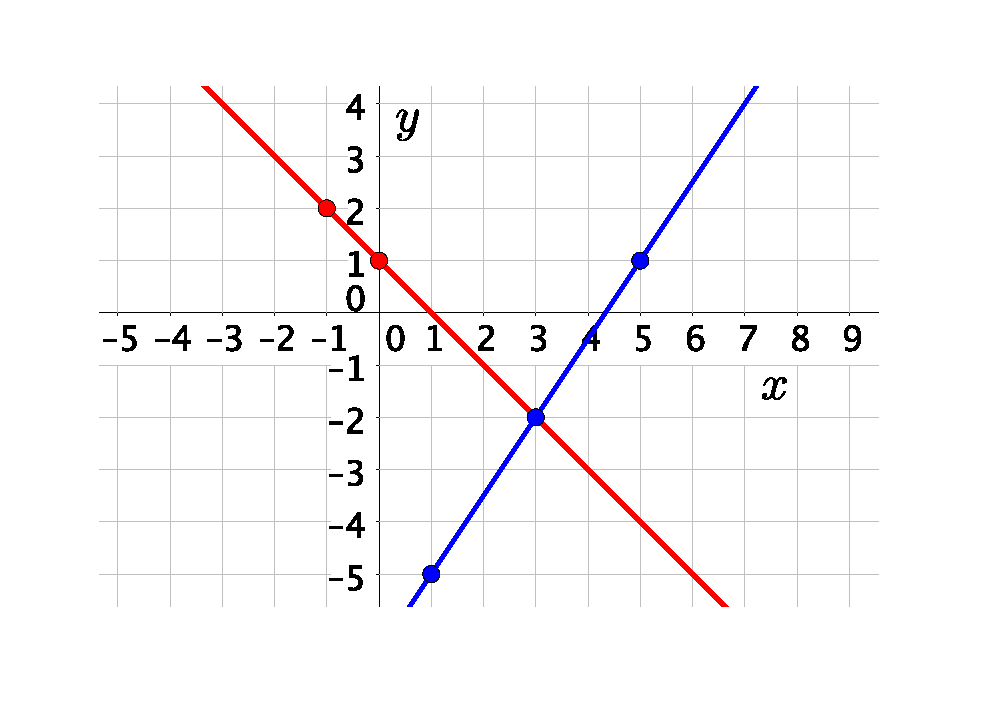
\includegraphics[width=5cm]{img-06/sistemagrafic}
	\end{center}
	 
	 
	\item	\textbf{ Comprovam la soluci\'o}: $\boxed{x=3,\ \ y=-2}$  Si substitu\"im $x$ i $y$ dins el sistema inicial s'han de complir les dues equacions a l'hora.
		
	\end{enumerate}	
	
\end{theorybox}

\begin{theorybox}
	Els sistemes es classifiquen en:
	
	\begin{multicols}{3}
	\centering
		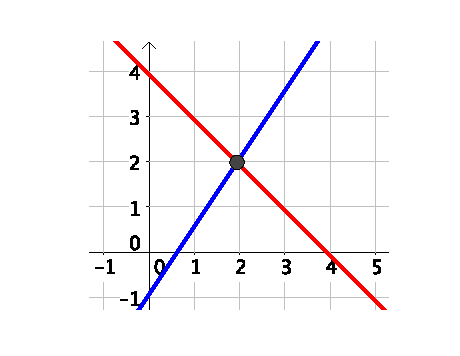
\includegraphics[width=3cm]{img-06/scd}
		
		1 solució - Compatible determinat
		
		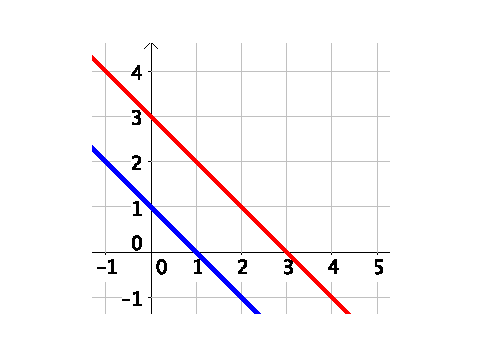
\includegraphics[width=3cm]{img-06/si}
		
		Cap solució - Incompatible
		
		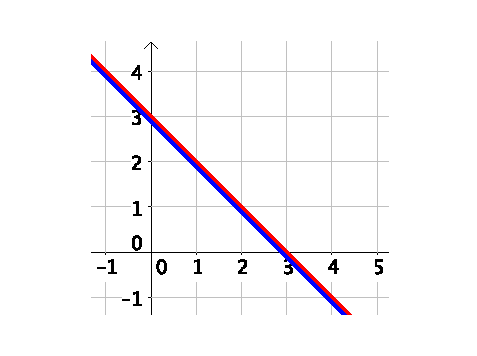
\includegraphics[width=3cm]{img-06/sci}
		
		Infinites solucions - Compatible indeterminat
	\end{multicols}
\end{theorybox}	
 
\newpage 

\begin{activitats}

\begin{mylist}

\exer  Resol les següents equacions de 2n grau

\begin{tasks}
	\task  $-$\textit{x}${}^{2}$ $-$ 6\textit{x} $-$ 8 = 0   
	\task  \textit{x}($-$ 1 + \textit{x}) = 6    
	\task  7\textit{x}${}^{2}$ = 70\textit{x}
	\task  2(\textit{x} + 3) $-$ \textit{x}(2\textit{x} + 1) = 5  
	\task  5(2\textit{x} $-$ 1) + \textit{x}(\textit{x} $-$ 1) = 5   
	\task \textit{ }12(\textit{x}${}^{2}$ $-$ 1) -- 6(2 + \textit{x}) = $-$ 18
	\task  (2\textit{x }+ 3)$\cdot$(\textit{x} $-$ 1) = $-$\textit{x} $-$ 3  
%	\task  \textit{x}$\cdot$(\textit{x} + 2) = 168   
	%\task  6(2\textit{x}${}^{2}$ $-$ 3\textit{x} + 1) $-$ \textit{x}(2\textit{x} -- 1) = --1
\end{tasks}
\answers{[$x=$--4 i --2, $x=$--2 i 3, $x=0$ i 10, $x=$--1/2 i 1, $x=$--10 i 1, $x=$--1/2 i 1, $x=$--1 i 0]}


\exer  Resol les següents equacions de 2n grau amb denominadors:

\begin{tasks}
	\task  $\frac{x^{2} -1}{2} -\frac{x+1}{3} =10$   
	\task   $\frac{x^{2} -3}{3} +\frac{x^{2} -x+1}{7} =3$  
	\task  $\frac{x^{2} +1}{5} +\frac{2x+6}{10} =2$
	\task  $\frac{1-x^{2} }{2} +\frac{3x-1}{3} =\frac{1}{3} $   
	\task  $\frac{2x^{2} -8}{5} -\frac{3x-9}{10} =x-1$  
	\task  $\frac{2x+3x^{2} }{5} -\frac{3x-6}{10} =1$
\end{tasks}
\answers{[$x=-\frac{13}{3}$ i 5, $x=-\frac{27}{10}$ i 3, $x=-3$ i 2, $x=\frac{3\pm \sqrt{6}}{3}$, $x=\frac{1}{4}$ i 3, $x=\frac{-1\pm\sqrt{97}}{12}$]}

\exer  Resol les següents equacions de 2n grau:

\begin{tasks}
	\task  \textit{x}${}^{2}$ $-$ 7\textit{x} + 10 = 0   
	\task  \textit{x}($-$1 + \textit{x}) = 0    
	\task  2\textit{x}${}^{2}$ = 50
	\task  \textit{x}${}^{2}$ $-$ 3\textit{x} $-$ 10 = 0   
	\task  \textit{x}${}^{2}$ + 3\textit{x} $-$ 10 = 0    
	\task  \textit{x}${}^{2}$ + 7\textit{x} + 10 = 0
	\task  \textit{x}${}^{2}$ $-$ 5\textit{x} + 6 = 0   
%	\task  \textit{x}${}^{2}$ $-$ \textit{x} $-$ 6 = 0     
%	\task  \textit{x}${}^{2}$ + \textit{x} $-$ 6 = 0
\end{tasks}
\answers{[$x=$,2 i 5 $x=$0 i 1, $x=\pm 5$, $x=$--2 i 5, $x=$--5 i 2, No té solució, $x=$2 i 3]}

\begin{comment}
\exer  Factoritza les equacions del problema anterior. Així, si les solucions són 2 i 5, escriu: 


\textit{x}${}^{2}$ $-$ 7\textit{x} + 10 = 0 \includegraphics*[bb=0 0 0.23in 0.17in, width=0.23in, height=0.17in, keepaspectratio=false]{img-06/image4.png} (\textit{x} -- 2)$\cdot$(\textit{x} -- 5) = 0.

Observa que si el coeficient de x${}^{ 2}$ fos diferent d'1 els factors han d'estar multiplicats per aquest coeficient.


\exer  Quan el coeficient \textit{b} és parell (\textit{b} = 2\textit{B}), pots simplificar la fórmula:  
\[x=\frac{-b\pm \sqrt{b^{2} -4ac} }{2a} =\frac{-2B\pm \sqrt{4B^{2} -4ac} }{2a} =\frac{-2B\pm 2\sqrt{B^{2} -ac} }{2a} =\frac{-B\pm \sqrt{B^{2} -ac} }{a} \] 


Així per resoldre \textit{x}${}^{2}$ $-$ 6\textit{x} + 8 = 0 basta dir $x=3\pm \sqrt{9-8} =3\pm 1$, i llavors les seves solucions són 2 i 4. Utilitza aquesta expressió per resoldre:

\begin{tasks}(2)
\task  \textit{x}${}^{2}$ $-$ 8\textit{x} $-$ 12 = 0   \task   \textit{x}${}^{2}$ $-$ 10\textit{x}  + 24 = 0    \task   \textit{x}${}^{2}$ + 4\textit{x} + 7 = 0
\end{tasks}

\end{comment}


\begin{comment}
\exer  Determina el nombre de solucions reals que tenen les següents equacions de segon grau calculant el seu discriminant, i després resol-les.

\begin{tasks}
	\task  \textit{x}${}^{2}$ + 3\textit{x} $-$ 4 = 0   
	\task  7\textit{x}${}^{2}$ + 12\textit{x} $-$ 4 = 0    
	\task  3\textit{x}${}^{2}$ + 7\textit{x} + 10 = 0
	\task  \textit{x}${}^{2}$ $-$ \textit{x} + 5 = 0   
	\task  6\textit{x}${}^{2}$ $-$ 2\textit{x} $-$ 3 = 0     
	\task  5\textit{x}${}^{2}$ + 8\textit{x} $-$ 6 = 0
\end{tasks}
\end{comment}


\exer  Escriu tres equacions de segon grau que no tinguin cap solució real. Ajuda: Utilitza el discriminant.
\answers{Per exemple, $x^2+1=0$, $x^2+x+1=0$ i $x^2-x+8=0$, cap d'elles tenen solució perquè els discriminants són $\Delta=-4$, $\Delta=-3$ i $\Delta=-31$ respectivament.}
\begin{comment}

\exer  Escriu tres equacions de segon grau que tinguin una solució doble.

\exer  Escriu tres equacions de segon grau que tinguin dues solucions reals i diferents.

\exer  Podries escriure una equació de segon grau amb únicament una solució real que no fos doble?
\end{comment}
\end{mylist}


 
\begin{mylist}


\exer  Resol els següents sistemes pel mètode de substitució:

\begin{tasks}
	\task  $\left\{\begin{array}{c} {2x-5y=-4} \\ {3x-y=7} \end{array}\right. $  
	\task  $\left\{\begin{array}{c} {3x+y=4} \\ {2x+5y=7} \end{array}\right. $  
	\task  $\left\{\begin{array}{c} {6x+5y=7} \\ {2x+3y=1} \end{array}\right. $
\end{tasks}
\answers{[$(3,2)$, $(1,1)$, $(2,-1)$]}

\exer  Resol els següents sistemes pel mètode d'igualació:

\begin{tasks}
	\task  $\left\{\begin{array}{c} {-2x+3y=13} \\ {3x-7y=-27} \end{array}\right. $  
	\task  $\left\{\begin{array}{c} {5x-2y=-3} \\ {4x-y=0} \end{array}\right. $  
	\task  $\left\{\begin{array}{c} {9x-5y=4} \\ {-8x+3y=-5} \end{array}\right. $
\end{tasks}
\answers{[$(-2,3)$, $(1,4)$, $(1,1)$]}


\exer  Resol els següents sistemes pel mètode de reducció:

\begin{tasks}
	\task  $\left\{\begin{array}{c} {3x-5y=1} \\ {2x+y=5} \end{array}\right. $   
	\task  $\left\{\begin{array}{c} {4x+3y=14} \\ {-x-6y=7} \end{array}\right. $  
	\task  $\left\{\begin{array}{c} {9x-5y=4} \\ {-7x+5y=-2} \end{array}\right. $
\end{tasks}
\answers{[$(2,1)$, $(5,-2)$, $(1,1)$]}


\exer  Copia en el teu quadern i completa els següents sistemes incomplets de manera que es compleixi el que es demana en cadascun:
\begin{tasks}
\task Compatible indeterminat 

 $\left\{\begin{array}{c} {\Box  x+3y=\Box } \\ {2x-y=3} \end{array}\right.$
\task  Incompatible 

 $\left\{\begin{array}{c} {-5x+y=2}  \\ {\Box x+y=6} \end{array}\right. $  
\task  La seva solució sigui $x = 2$ i $y = 1$ 

$\left\{\begin{array}{c} {3x-y=\Box } \\ {\Box x+y=7} \end{array}\right. $
\task   Compatible indeterminat 

$\left\{\begin{array}{c} {\Box x+6y=\Box }\\ {2x+3y=-2} \end{array}\right. $
\end{tasks}
\answers{[$\Box=$--6 i --9, $\Box=$--5, $\Box=$5 i 3, $\Box=$4 i --4]}
 


\exer  Resol els següents sistemes pel mètode que creguis més convenient:

\begin{tasks}
	\task  $\left\{\begin{array}{c} {\frac{4x-1}{3} -\frac{2y+2}{5} =-1} \\ {\frac{x+3}{2} +\frac{4y-1}{3} =7} \end{array}\right. $   
	\task  $\left\{\begin{array}{c} {\frac{3x-1}{2} -\frac{y+3}{5} =-3} \\ {3x+y=-1} \end{array}\right. $  
	\task  $\left\{\begin{array}{c} {\frac{x+1}{2} +\frac{y+2}{3} =2} \\ {3x-2y=1} \end{array}\right. $
\end{tasks}
\answers[cols=1]{[Sistema:\par $\left\{ \begin{array}{l} 10x-3y=-2\\ 3x+8y=35 \end{array} \right.$. Solució: $(1,4)$, 
	Sistema:\par $\left\{ \begin{array}{l} 15x-2y=-19 \\ 3x+y=-1 \end{array} \right.$. Solució: $(-1,2)$, 
	Sistema:\par $\left\{ \begin{array}{l} 3x+2y=5 \\ 3x-2y=1 \end{array} \right.$. Solució: $(1,1)$]}

\begin{comment}
\exer  Escriu tres sistemes lineals que siguin incompatibles.

\exer  Escriu tres sistemes lineals que siguin compatibles indeterminats.

\exer  Escriu tres sistemes lineals que siguin compatibles determinats.

\end{comment}

\exer  Resol els següents sistemes pel mètode d'igualació i comprova la solució gràficament. De quin tipus és cada sistema?

\begin{tasks}
	\task  $\left\{\begin{array}{c} {-2x+6y=13} \\ {x-3y=8} \end{array}\right. $   
	\task  $\left\{\begin{array}{c} {x-y=-3} \\ {4x-4y=-12} \end{array}\right. $   
	\task  $\left\{\begin{array}{c} {x-y=4} \\ {-x+3y=-5} \end{array}\right. $
\end{tasks}
\answers{[Incompatible, Compatible indeterminat,  Compatible determinat $x = 9/2$, $y = –1/2$]}

 
\exer  En una botiga lloguen bicicletes i tricicles. Si tenen 51 vehicles amb un total de 133 rodes, quantes bicicletes i quants tricicles tenen?
\answers{$x=$Bicicletes , $y=$Tricicles. Planteig: $\left\{\begin{array}{l}
	 x+y=51\\
 2x+3y=133\\
	\end{array} \right.$. Solució: $x=20$ bicicletes  i $y=31$ tricicles }

\exer  Quina és l'edat d'una persona si en multiplicar-la per 15 li falten 100 unitats per completar el seu quadrat?
\answers{$15x+100=x^2$, $x=20$ anys}

%\exer  Descompon 8 en dos factors que la seva suma sigui 6

%\exer  El triple del quadrat d'un nombre augmentat en el seu doble és 85. Quin nombre és?

\exer  La suma dels quadrats de dos nombres imparells consecutius és 394. Determina aquests nombres. 
\answers{$(2x-1)^2+(2x+1)^2=394$. Els nombres són --15 i 13; o bé 13 i 15}

\exer  Van carregats un ase i un mul. L'ase es queixava del pes que portava damunt. El mul li va contestar: Si jo portés un dels teus sacs, portaria el doble de càrrega que tu, però si tu prens un dels meus, els dos portarem igual càrrega. Quants sacs porta cadascun?
\answers{$x=$Ase , $y=$Mul. Planteig: $\left\{\begin{array}{l}
	y+1=2(x-1)\\
	y-1=x+1\\
	\end{array} \right.$. Solució: $x=5$ ase  i $y=7$ mul (sacs) }

%\exer  Quin nombre multiplicat per 3 és 40 unitats menor que el seu quadrat?

\exer  Calcula tres nombres consecutius que la seva suma de quadrats és 365
\answers{$x+(x+1)^2+(x+2)^2=365$. Els nombres són --12, --11,--10 o bé 10, 11, 12.}

\exer  D'aquí d'11 anys, l'edat de'n Mario serà la meitat del quadrat de l'edat que tenia fa 13 anys. Quina edat té Mario?
\answers{$x:$ edat actual de'n Mario. $x+11=\frac{(x-13)^2}{2}$. Mario té 21 anys.}

%\exer  Dos nombres naturals es diferencien en 2 unitats i la suma dels seus quadrats és 580. Quins són aquests nombres?

\exer  La suma de dos nombres és 5 i el seu producte és $-$84. De quins nombres es tracta?
\answers{$x=$,$y=$els nombres. Planteig: $\left\{\begin{array}{l}
	x+y=5\\
	x\cdot y=-84\\
	\end{array} \right.$. Solució: $x=12$; $y=-7$  i viceversa.}

\exer  Maria vol formar safates d'un quilogram amb massapans i polvorons. Si els polvorons li costen a 5 euros el quilo i els massapans a 7 euros el quilo, i vol que el preu de cada safata sigui de 6 euros, quina quantitat haurà de posar de cada producte? Si vol formar 25 safates, quina quantitat de polvorons i de massapans necessitarà?
\answers{$x=$kg polvorons, $y=$kg massapà. Planteig: $\left\{\begin{array}{l}
	x+y=1\\
	5x+7y=6\\
	\end{array} \right.$. Solució: A cada safata: $x=0.5$ kg de polvorons  i $y=0.5$ kg de massapà. En total necessitarà $12.5$ kg de cada producte.}

\exer  Determina els catets d'un triangle rectangle que la seva suma és 7 cm i la hipotenusa d'aquest triangle mesura 5 cm.
\answers{$x=$,$y=$catets. Planteig: $\left\{\begin{array}{l}
	x+y=7\\
	x^2+y^2=25\\
	\end{array} \right.$. Solució: $x=3$  i $y=4$ (o viceversa) }

\exer  El producte de dos nombres és 4 i la suma dels seus quadrats 17. Calcula aquests nombres
\answers{$x=$,$y=$els nombres. Planteig: $\left\{\begin{array}{l}
	x\cdot y = 4\\
	x^2+y^2=17\\
	\end{array} \right.$. Solució: $x=-4$, $y=-1$ o viceversa, o  $x=1$, $y=4$ o viceversa. En total 4 solucions. }

%\exer  La suma de dos nombres és 20. El doble del primer més el triple del segon és 45. De quins nombres es tracta?

\exer  En un garatge hi ha 30 vehicles entre cotxes i motos. Si en total hi ha 100 rodes, quants cotxes i motos hi ha en el garatge?
\answers{$x=$cotxes , $y=$motos. Planteig: $\left\{\begin{array}{l}
	x+y=30\\
	4x+2y=100\\
	\end{array} \right.$. Solució: $x=20$ cotxes  i $y=10$ motos}

\exer  L'edat actual d'en Pere és el doble de la de Raquel. D'aquí de 10 anys, les seves edats sumaran 65. Quants anys tenen actualment en Pere i na Raquel?
\answers{$x=$Edat Pere, $y=$Edat Raquel. Planteig: $\left\{\begin{array}{l}
	x=2y\\
	x+10+y+10=65\\
	\end{array} \right.$. Solució: $x=30$ anys Pere  i $y=15$ Raquel  }

\exer  En la meva classe hi ha 35 persones. Ens han regalat a cada nina 2 bolígrafs i a cada nin 1 quadern. Si en total hi havia 55 regals. Quants nins i nines som en classe?
\answers{$x=$Nines , $y=$Nins. Planteig: $\left\{\begin{array}{l}
	x+y=35\\
	2x+y=55\\
	\end{array} \right.$. Solució: $x=20$ nines  i $y=15$ nins }

\exer  Entre el meu avi i el meu germà tenen 56 anys. Si el meu avi té 50 anys més que el meu germà, quina edat té cadascun?
\answers{$x=$Edat avi , $y=$Edat germà. Planteig: $\left\{\begin{array}{l}
	x+y=56\\
	x=50+y\\
	\end{array} \right.$. Solució: $x=53$ anys l'avi  i $y=3$ el germà }

\exer  Dos entrepans i un refresc costen 5€. Tres entrepans i dos refrescs costen 8€. Quin és el preu de l'entrepà i el refresc?
\answers{$x=$\euro{} Entrepà , $y=$\euro{}  Refresc. Planteig: $\left\{\begin{array}{l}
	2x+y=5\\
	3x+2y=8\\
	\end{array} \right.$. Solució: $x=2$ \euro{} entrepà  i $y=1$ el refresc}

\exer  En una granja hi ha pollastres i vaques. Si es compten els caps, són 50. Si es compten les potes, són 134. Quants pollastres i vaques hi ha en la granja?
\answers{$x=$Pollastres, $y=$vaques. Planteig: $\left\{\begin{array}{l}
	x+y=50\\
	2x+4y=134\\
	\end{array} \right.$. Solució: $x=33$ pollastres  i $y=17$ vaques}

%\exer  Un rectangle té un perímetre de 172 metres. Si el llarg és 22 metres major que l'ample, quines són les dimensions del rectangle?

\exer  En una bossa hi ha monedes de 1€ i 2€. Si en total hi ha 40 monedes i 53€, quantes monedes de cada valor hi ha en la bossa?
\answers{$x=$monedes de 1, $y=$monedes de 2. Planteig: $\left\{\begin{array}{l}
	x+y=40\\
	x+2y=53\\
	\end{array} \right.$. Solució: $x=27$ monedes d'1\euro{}  i $y=13$  de 2 \euro{}}

\columnbreak

\exer  En una baralla entre aranyes i vespes, hi ha 70 caps i 488 potes. Sabent que una aranya té 8 potes i una vespa 6, quantes vespes i aranyes hi ha en la baralla?
\answers{$x=$aranyes , $y=$vespes. Planteig: $\left\{\begin{array}{l}
	x+y=70	\\
	8x+6y=488\\
	\end{array} \right.$. Solució: $x=34$ aranyes  i $y=36$ vespes.}
%\exer  Una classe té 32 estudiants, i el nombre nines és triple al de nins, quants nins i nines hi ha?

\exer  Iolanda té 6 anys més que el seu germà Pau, i la seva mare té 50 anys. D'aquí 2 anys, l'edat de la mare serà doble de la suma de les edats dels seus fills. Quines edats tenen?
\answers{$x=$edat actual Iolanda, $y=$edat actual Pau. Planteig: $\left\{\begin{array}{l}
	x = y +6\\
	52 = 2 ( x+2 \, +\, y+2 )\\
	\end{array} \right.$. Solució: $x=14$ anys Iolanda  i $y=8$ Pau }

\end{mylist}
\end{activitats}

 
 
\begin{autoaval}{40}
	\begin{mylist}

\exer[2] Resol l'equació 3(\textit{x}${}^{2}$ -- 1) + 2(\textit{x}${}^{2}$ -- 2\textit{x}) = 9.
\begin{comment}
\begin{tasks}(4)
\task  \textit{x} = 2 i \textit{x} = 1   
\task  \textit{x} = 1 i \textit{x} = --3 
\task  \textit{x} = 1 i \textit{x} = --2/3  
\task  \textit{x} = 2 i \textit{x} = --6/5
\end{tasks}
\end{comment}
\answers{$x=2$ i $x=-6/5$}

\exer[2] Resol 156 = \textit{x}(\textit{x} -- 1) 
\begin{comment}
\begin{tasks}(4)
	\task  \textit{x} = 11 i \textit{x} = --13  
	\task  \textit{x} = 13 i \underbar{x} = --12  
	\task  \textit{x} = 10 i \textit{x} = 14  
	\task  \textit{x} = --12 i \textit{x} = --11
\end{tasks}
\end{comment}
\answers{$x=13$ i $x=-12$}

\exer[2] Resol l'equació 3x${}^{ 2}$ -- 14x + 15 = 0  
\begin{comment}
\begin{tasks}(4)
	\task  \textit{x} = 2 i \textit{x} = 2/3  
	\task  \textit{x} = 1/3 i \textit{x} = 4  
	\task  \textit{x} = 1 i \textit{x} = 4/3  
	\task  x = 5/3 i \textit{x} = 3
\end{tasks}
\end{comment}
\answers{$x=5/3$ i $x=3$}

\exer[2] Resol l'equació (\textit{x} -- 14)${}^{2}$ + \textit{x}${}^{2}$ = (\textit{x} + 2)${}^{2}$ 
\begin{comment} 
\begin{tasks}(4)
	\task  \textit{x} = 24 i \textit{x} = 8  
	\task  \textit{x} = 21 i \textit{x} = 3  
	\task  \textit{x} = 5 i \textit{x} = 19  
	\task  \textit{x} = 23 i \textit{x} = 2
\end{tasks}
\end{comment}
\answers{$x=24$ i $x=8$}

\exer[2] Resol l'equació $2(x+2)-x(2-x)=0$ 
\begin{comment}
\begin{tasks}(4)
	\task  Infinites   
	\task  \textit{x} = 9 i \textit{x} = 5   
	\task  no té solució  
	\task  \textit{x} = 1 i \textit{x} = 4
\end{tasks}
\end{comment}
\answers{No té solució}

\exer[2] Com són les rectes que formen el sistema $\left\{\begin{array}{c} {2x+3y=3} \\ {5x-4y=9} \end{array}\right. $ ?
\begin{comment}
\begin{tasks}(4)
	\task  Secants   
	\task  Paral·leles   
	\task  Coincidents  
	\task  Es creuen
\end{tasks}
\end{comment}
\answers{Secants}

\exer[2] Resol el sistema $\left\{\begin{array}{c} {3x-4y=2} \\ {6x-8y=12} \end{array}\right. $ 
\begin{comment}
\begin{tasks}(4)
	\task  \textit{x} = 2 i \textit{y =} 1   
	\task  \textit{x} = 1 i \textit{y =} 1   
	\task  \textit{x} = 3 i \textit{y =} 2   
	\task  No té solució
\end{tasks}
\end{comment}
\answers{No té solució}

\exer[2] Resol el sistema $\left\{\begin{array}{c} {3x+4y=2} \\ {5x-y=11} \end{array}\right. $
\begin{comment}
\begin{tasks}(4)
	\task  \textit{x} = 4 i \textit{y =} 2   
	\task  \textit{x} = 3 i \textit{y =} 3   
	\task  \textit{x} = 2 i \textit{y =} $-$1   
	\task  \textit{x} = 5 i \textit{y =} 1
\end{tasks}
\end{comment}
\answers{$x=2$ i $y=-1$}

\exer[2] En una granja, entre pollastres i porcs hi ha 27 animals i 76 potes. Quants pollastres i porcs hi ha en la granja?
\begin{comment}
\begin{tasks}(3)
	\task  16 pollastres i 11 porcs     
	\task  15 pollastres i 12 porcs        
	\task  13 pollastres i 14 porcs
\end{tasks}
\end{comment}
\answers{16 pollastres i 11 porcs}

\exer[2] Quina és l'edat d'una persona si en multiplicar-la per 15, li falten 100 unitats per arribar al seu quadrat?
\begin{comment}
\begin{tasks}(4)
	\task  16 anys   
	\task  17 anys   
	\task  20 anys   
	\task  18 anys 
\end{tasks}
\end{comment}
\answers{20 anys}
 
\end{mylist}
\end{autoaval}


\pagebreak
\vspace*{-1cm}
\resum
\begin{center}
	\renewcommand{\arraystretch}{1.1}

\begin{longtable}{|P{0.2\textwidth}|p{0.38\textwidth}|p{0.38\textwidth}|} \hline 
	
\cellcolor{lightgray}\textbf{Equació de primer grau} & És una equació algebraica en la qual la major potència de la incògnita és 1. & $-$ 5\textit{x} + 6 = 0\textit{} \\ \hline 

\cellcolor{lightgray}\textbf{Equació de segon grau} & És una equació algebraica en la qual la major potència de la incògnita és 2. Té la forma: \textit{ax}${}^{2}$ + \textit{bx} + \textit{c} = 0, on \textit{a, b } i \textit{ c} són nombres reals, amb $a\neq 0$. & $-$3\textit{x}${}^{2}$ + 7\textit{x} $-$8 = 0 \\ \hline

\cellcolor{lightgray} \textbf{Resolució d'equacions de 2n grau completes} & S'utilitza la fórmula:\par $x=\frac{-b\pm \sqrt{b^{2} -4ac} }{2a} $ & $x^2-5x+6=0$:\par  $x=\frac{5\pm \sqrt{25-4\cdot 1\cdot 6} }{2\cdot 1} =\frac{5\pm 1}{2} $ \par $x_1=3$, $x_2=2$ \\ \hline

\cellcolor{lightgray} \textbf{Discriminant} & $\Delta$ = \textit{b}${}^{2}$\textit{ }-- 4\textit{ac} & $\Delta$ = ($-$5)${}^{2}$ $-$ 4$\cdot$1$\cdot$6 = 25 $-$24 =1 \\  \hline 

\cellcolor{lightgray}\textbf{Nombre de solucions d'una equació de 2n grau} & Si $\Delta$  = \textit{b}${}^{2}$\textit{ }-- 4\textit{ac} $>$ 0, té dues solucions reals i diferents\newline Si $\Delta$  = \textit{b}${}^{2}$\textit{ }-- 4\textit{ac} = 0, té una solució doble.\newline Si $\Delta$  = \textit{b}${}^{2}$\textit{ }-- 4\textit{ac} $<$ 0, l'equació no té solució & \textit{x}${}^{2}$ $-$ 4\textit{x} $-$ 5 = 0: $\Delta$ =36 $>$ 0, té dues solucions 5 i $-$1.\newline \textit{x}${}^{2}$ $-$ 2\textit{x} + 1 = 0: $\Delta$ = 0, té una arrel doble: \textit{x} = 1.\newline \textit{x}${}^{2}$ + 3\textit{x} + 8 = 0: $\Delta$ = $-$23. No té solució real \\ \hline 

\cellcolor{lightgray}\textbf{Resolució d'equacions de 2n grau incompletes} & Si \textit{b} = 0, \textit{ax}${}^{2}$ + \textit{c} = 0, buidem la incògnita: $x=\pm \sqrt{\frac{-c}{a} } $.\newline Si \textit{c} = 0, \textit{ax}${}^{2}$ + \textit{bx} = 0: \textit{x} = 0 i $x=\frac{-b}{a} $ & 2\textit{x}${}^{2}$ $-$ 18 = 0:\textbf{\textit{ $x=\pm \sqrt{9} =\pm 3$\newline }}\newline 3\textit{x}${}^{2}$ $-$ 15\textit{x} = 0 $\Rightarrow$ 3\textit{x}(\textit{x} -- 5) = 0 $\Rightarrow$ \newline \textit{x${}_{1}$} = 0; \textit{x${}_{2}$} = 5. \\\hline 

\cellcolor{lightgray}\textbf{Suma i producte d'arrels} & \textit{x}${}_{1}$\textit{ x}${}_{2}$ = $\frac{c}{a} $; \textit{x}${}_{1}$ +\textit{ x}${}_{2}$ = $\frac{-b}{a} $ & \textit{x}${}^{2}$ $-$ 5\textit{x} + 6 = 0 $\Rightarrow$ \textit{x${}_{1}$}= 2; \textit{x${}_{2}$}= 3 \\ \hline 

\cellcolor{lightgray}\textbf{Sistema d'equacions} & $\left\{\begin{array}{c} {ax+by=c} \\ {a'x+b'y=c'} \end{array}\right. $ & $\left\{\begin{array}{c} {x+2y=3} \\ {7x-3y=4} \end{array}\right. $ \\\hline 

\cellcolor{lightgray}\textbf{Classificació} & \multicolumn{2}{|p{3.8in}|}{\textbf{Compatible determinat}: Una única solució, el punt d'intersecció. Les rectes són \textbf{secants}:\newline  $\left\{\begin{array}{c} {x+3y=4} \\ {-2x+y=-1} \end{array}\right. $\newline \textbf{Compatible indeterminat}: Infinites solucions, per la qual cosa les rectes són \textbf{coincidents: }$\left\{\begin{array}{c} {x-3y=3} \\ {2x-6y=6} \end{array}\right. $\textbf{\newline Incompatible}: No té solució, les rectes són \textbf{paral·leles: $\left\{\begin{array}{c} {x-3y=3} \\ {2x-6y=2} \end{array}\right. $\newline }}\\ \hline 

\cellcolor{lightgray}\textbf{Mètodes de resolució} & \multicolumn{2}{|p{0.75\textwidth}|}{\textbf{Substitució:} aïllar una incògnita i substituir en l'altra equació. \newline \textbf{Igualació:} aïllar la mateixa incògnita de les dues equacions.\newline \textbf{Reducció:} sumar les dues equacions, multiplicant-les per nombres adequats.\newline \textbf{Gràficament}: representar les dues funcions lineals i determinar el punt $(x, y)$ on es tallen}\\ \hline 
\end{longtable}
\end{center}


 




